During this section we will describe the way we have chosen to implement a system of transcribing a sequence of beatboxing into a form that can be easily interpreted. The subsections will first off go through the perimeters of what will be transcribed, namely what beatboxing sounds will be analysed on. Secondly a section about data collection will talk about how we have gathered data both for use in the implementation of the system and in the evaluation of the systems performance. When the data has been collected, the actual transcription system can be implemented and will here be described. This is divided into three parts: first how the system will segment audio in order to analyse it, then the analysis of the segmentation, i.e. feature extraction and classification, and finally a presentation of an application with a user interface.

All implementation of the system is done through Matlab\footnote{\url{http://www.mathworks.se/products/matlab/}} using its built-in scripting system. This allows for easy analysis and processing of digital signals.


\section{Choosing Sound Classes}
Based on some of the previous works by \cite{Stowell2010} and \cite{QBBB} a set of 3 basic beatboxing sounds have been chosen for this experiment. The first of them is the kick drum, which is also known as the base drum because of its deep-sounding nature. The spectrum of the kick drum lies in the lower frequencies as seen in figure \ref{fig:kick-wave}. The second sound is the snare drum and we have been focussing on the k-snare as opposed to the p-snare, which is performed with an initial k-sound. Lastly the hi-hat cymbal was chosen, which has a frequency spectrum a bit higher than the snare as can be seen in figure \ref{fig:snare-wave} and \ref{fig:hihat-wave}.

\begin{figure}[h]
	\centering
	\begin{subfigure}[b]{0.275\textwidth}
		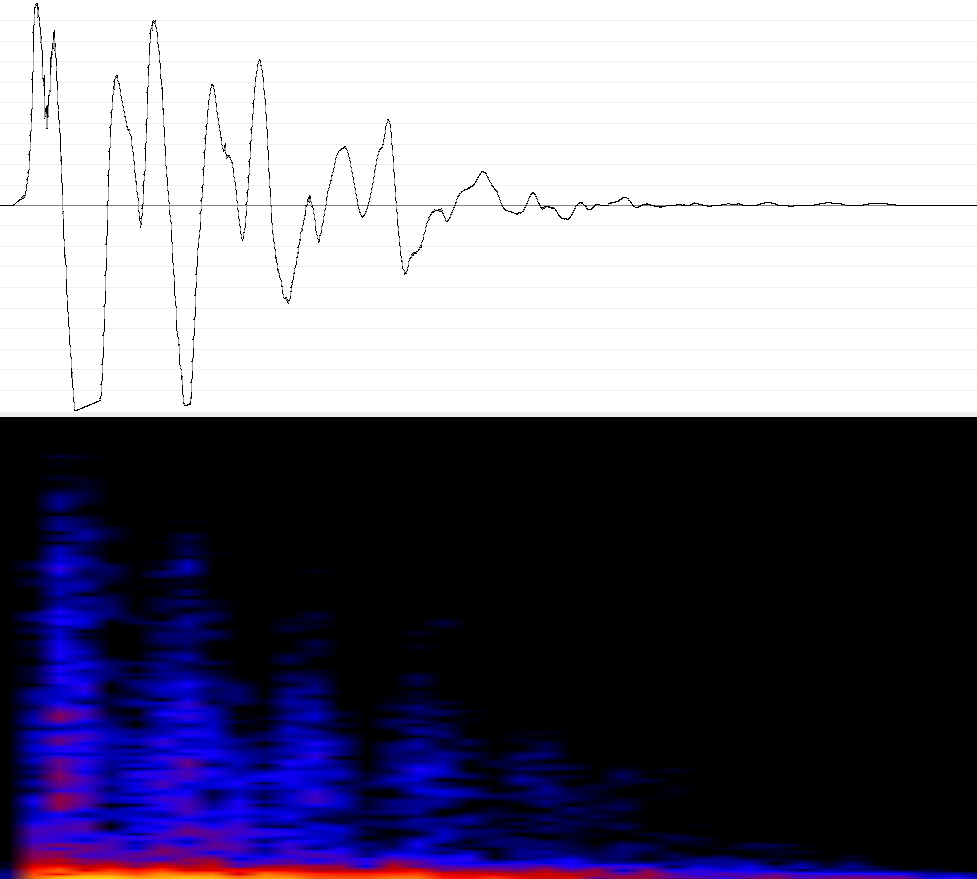
\includegraphics[width=\textwidth]{fig/Kick-wave.png}
		\caption{Kick drum}
		\label{fig:kick-wave}
	\end{subfigure}
	\begin{subfigure}[b]{0.275\textwidth}
		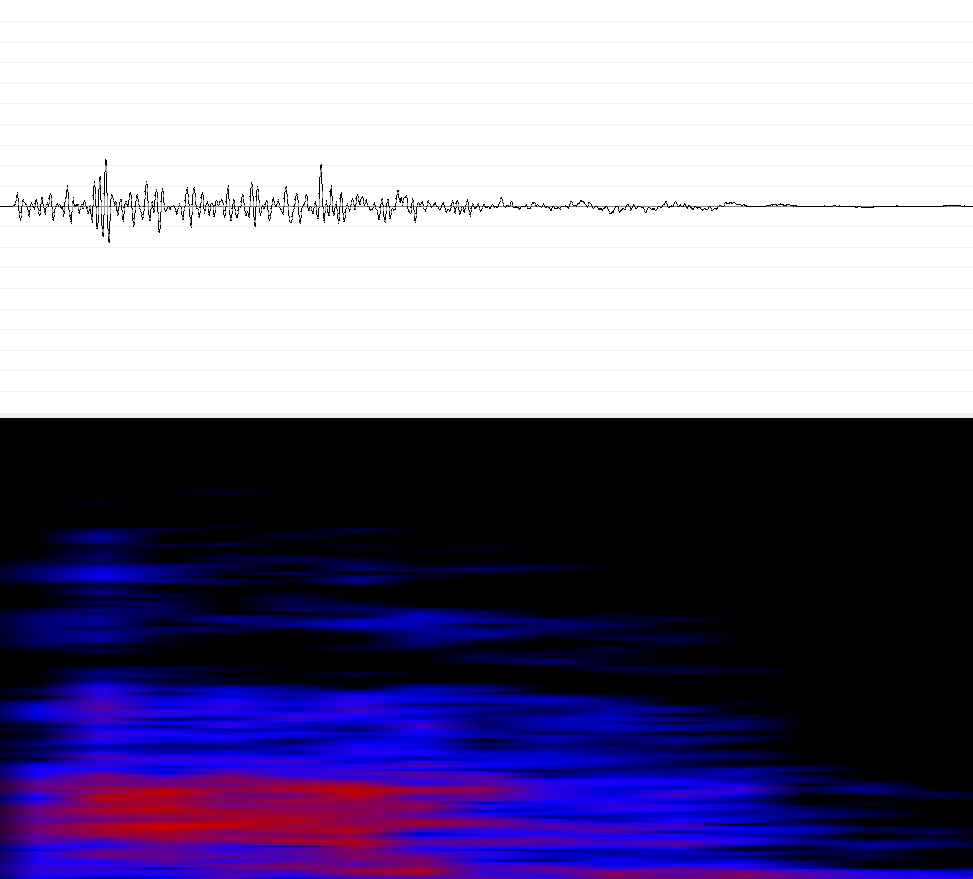
\includegraphics[width=\textwidth]{fig/Snare-wave.png}
		\caption{Snare drum}
		\label{fig:snare-wave}
	\end{subfigure}
	\begin{subfigure}[b]{0.35\textwidth}
		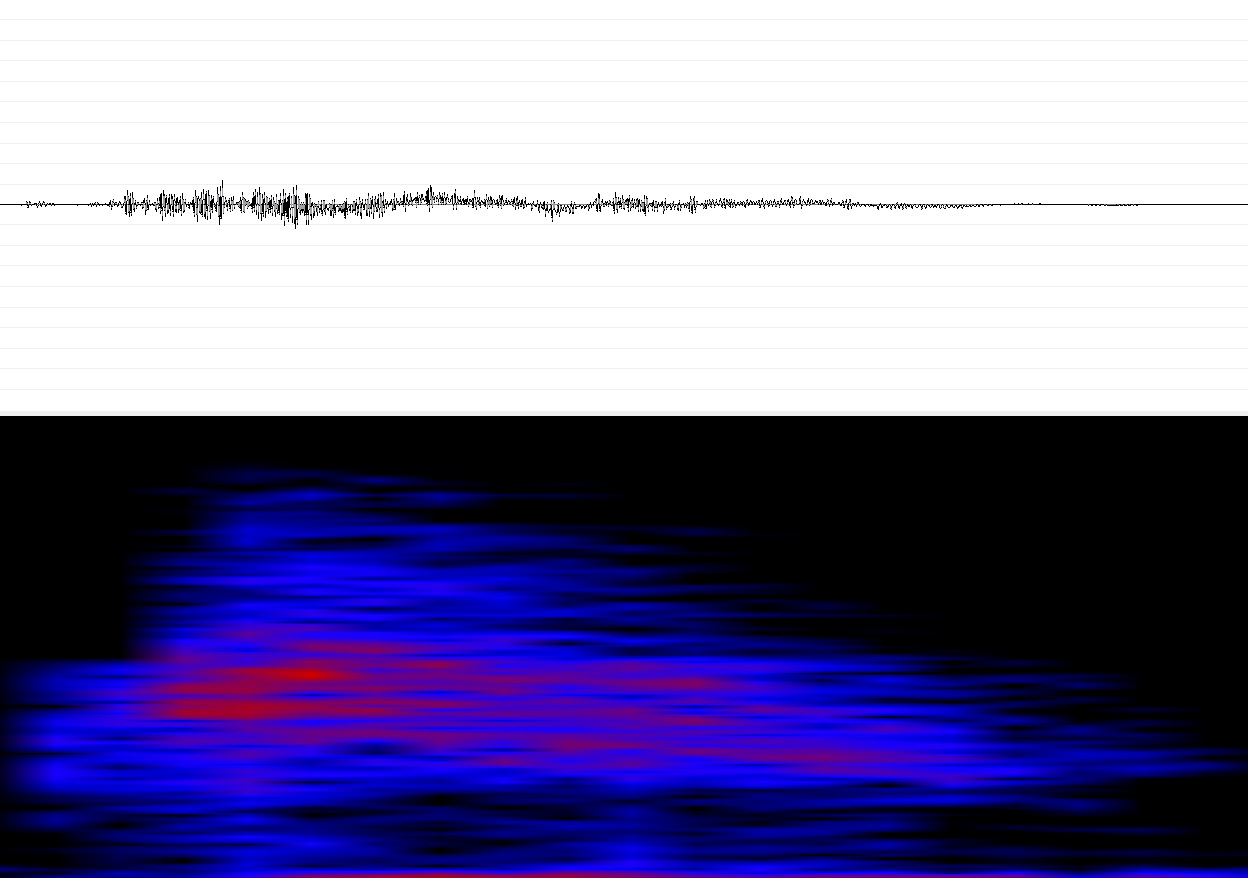
\includegraphics[width=\textwidth]{fig/Hihat-wave.png}
		\caption{Hi-hat}
		\label{fig:hihat-wave}
	\end{subfigure}
	\caption{A presentation of 3 beatboxing sounds' waveform (top) and spectrogram
	\label{fig:chosen-sounds} (bottom).}
\end{figure}

What we can see from these waveforms and spectra is that the kick drum does differ significantly in its frequency content in relation to the snare and hi-hat. The snare and hi-hat does initially seem to have a clear difference in their frequencies, however they do not seem to lie in a very concentrated area of the spectrum, indicating that they might prove difficult to distinct from each other based on the frequency content.
\section{Collection of dataset}
This chapter will go through how a dataset was collected containing only some specific beat boxing sounds.
For collection of the dataset containing beat boxing, only three type of different beat boxing sounds there was made use of a recorder, a microphone, a headset, some boards (to limit the noise from surroundings as much as possible) and a computer to take notes of when the different people did record their beat boxing, The setup of the place where the record took place and be seen on figure \ref{data-collection-pic}. For choosing the people to help us make the beatboxing random convenience method was used. 
\begin{figure}[h]
	\begin{center}
		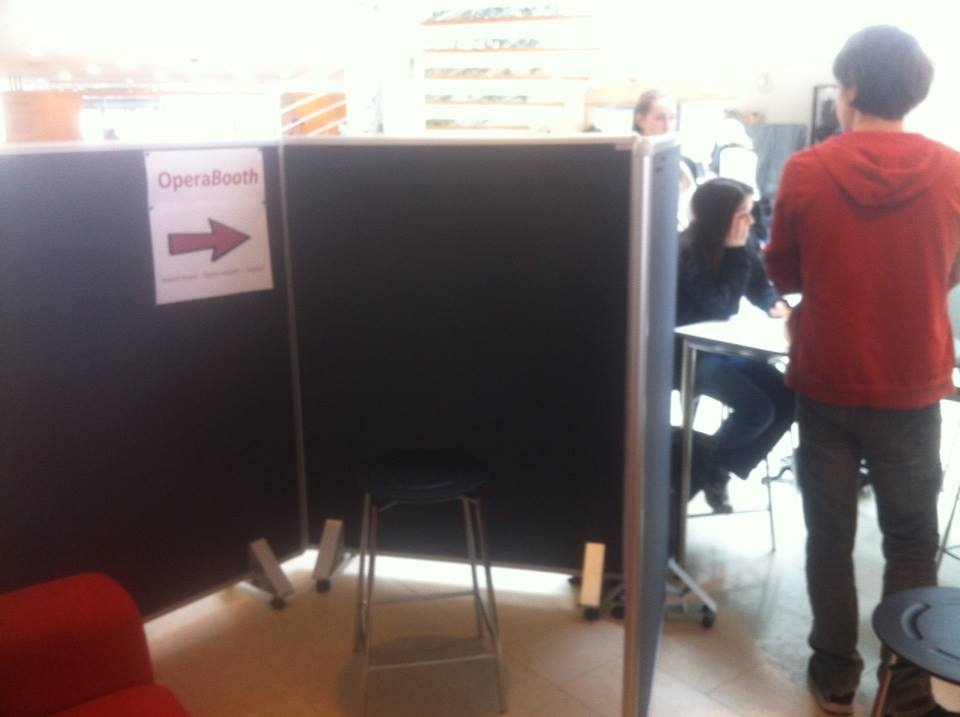
\includegraphics[height=5cm]{fig/dataset_collection.JPG}
		\caption{data-collection-pic}
		\label{data-collection-pic}
	\end{center}
\end{figure}
When the participants sat in the stall they was asked to practice a few different beat boxing sounds, when they had learned one they would be recorded making that  sound this was repeated with three sounds, a kick drum beat boxing sound, a snare drum beat boxing sound and a hi-hat drum beat boxing sound. After they had made the three sounds they were also asked to improvise a short mix of the three beat boxing sounds that they had learned.

\section{Segmentation}
This section will go through how the segmentation of the sound was achieved. The segmentation is needed to locate each sound's endpoints in a signal, i.e. the positions in time at which each sound starts and ends. This is a necessary part of the transcription system as we need to be able to distinct the sounds from each other and not the whole signal as a combination of many sounds.

In this transcription system the segmentation is made by calculating the logarithm of the RMS of each window and if this value, from one window to the next, goes above a threshold it is considered as the starting point of a sound. Similarly when the value falls below the threshold the end of the sound is registered.

The MATLAB function for segmenting the signal analyses the signal using a specified window size and window skip. When all endpoints in the signal are found, a cell array is returned containing the signal divided into segments so that each cell contains the frames for that segment.

\begin{figure}[h]
	\begin{center}
		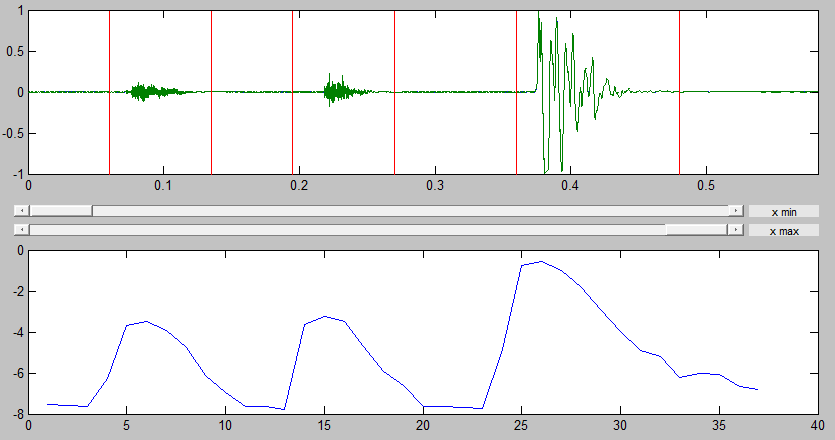
\includegraphics[scale =  0.4]{fig/SegmentationPic.png}
		\caption{An example of how the signal will be segmented. On the top the signal is plotted in the time domain with vertical lines indicating the segmentation points (endpoints). The bottom shows the logarithm of the RMS to the signal from above.}
		\label{SegmentationPic}
	\end{center}
\end{figure}

An example of the result from this segmentation is shown in figure \ref{SegmentationPic}. At the top we see the input signal and vertical lines indicating the endpoints of each segment. On the bottom of the figure a graph of the change in the logarithm of the RMS is plotted where we see a peak at each segment in the signal.
\section{Features}
All feature extraction should be usable independently of each other, thus each calculation of the features is implemented in its own function that will return one or more values about that feature. In the following we have divided the description of the features in 3 categories: the time domain features, spectral domain features and the MFCC in its own category.

% TIME DOMAIN SUBSEC ---- START
\subsection{Time Domain Features}
The time domain features consisting of the Root Mean Square (RMS) and Zero-Crossings (ZC) are implemented as functions that each takes the signal or just a segment as input. The RMS function will return a value indicating what the mean energy of the input is, while the total number of zero-crossings will be returned from the ZC function. Programmatically the implementation is rather simple, as can be seen in figure \ref{snippet-RMS} and \ref{snippet-ZC}, where a single loop iterates through all input samples to calculate the output.

\begin{lstlisting}[caption=Matlab implementation of the RMS algorithm., label=snippet-RMS]
function rms = P4_RMS(x)
    % rms = P4_RMS(x)
    %
    % @param x: signal vector.
    % @retval: returns the root mean square of the signal x.
    rms = 0;
    for ii = 1:length(x)
       rms = rms + x(ii)^2; 
    end
    rms = sqrt(rms / length(x));
end
\end{lstlisting}

\begin{lstlisting}[caption=Matlab implementation of the ZC algorithm., label=snippet-ZC]
function zc = P4_zero_crossing(signal)
    % zc = P4_zero_crossing(x)
    %
    % @param x: signal vector.
    % @retval Returns the total zero crossings of the signal x.
    zc = 0;
    for ii = 2:length(signal)
        if (signal(ii) * signal(ii-1) < 0)
            zc = zc + 1;
        end
    end
end
\end{lstlisting}
% TIME DOMAIN SUBSEC ---- END

% SPECTRAL DOMAIN SUBSEC ---- START
\subsection{Spectral Domain Features}
Spectral domain features uses the information gathered in a spectrogram of the sound. Before being able to actually do any calculations of the spectral features, the spectrogram needs to be produced. Using the built-in function in Matlab for calculating the Fast Fourier Transform (FFT) we can produce a spectrogram of the input sound/segment by looping over the input using the specified window size and skip, see appendix \ref{app:feat-spectrogram}. This spectrogram will then be forwarded to the function corresponding to each of the spectral feature-calculations implemented as follows.

The spectral features implemented are: (a) Centroid, (b) Flux, (c) Rolloff and (d) Skewness, all of which are implemented using the code provided by Alexander Lerch\footnote{\url{http://www.audiocontentanalysis.org/code/}} \citep{ACA}. The extracted value from each of these features is a mean value of the whole signal segment sent into the function. This value is directly used in the classifier to identify and describe that specific segment. See appendices under \ref{app:features} for complete implementation.
% SPECTRAL DOMAIN SUBSEC ---- END

\subsection{Mel Frequency Cepstral Coefficients}
Using the MFCC algorithm provided by Malcolm Slaney we have implemented a version of it that has been adjusted by Bob L. Sturm. This adjustment makes it possible to use different analysis window sizes and skips, please refer to provided Matlab-script "mfcc.m". The algorithm will provide a feature vector with 40 cepstral coefficients that describe every window of the input sound. To use these coefficients, we take a mean over all windows, i.e. for every coefficient we take the mean value of that coefficient over all windows. Out of these 40 mean values, we use the first 20 coefficients.
\\

\colorbox{red}{WE NEED kNN HERE}
\section{Classification using Nearest Neighbour}
This chapter will give information on the classification method called KNN (K nearest neighbour).

Shortly put in \citep{meaningfulNN} the NN is "given a collection of data point and query points in an m-dimentional metric space, find the data point that is closets to the query point".

If going into more detail the above sentence will mean that the NN classification will need a dataset that can train a system \citep{Sinoyr05}, the data used for training has to be notated so that the program that make the classification knows what the different data represent. When one has trained the data they need some value to describe what sound it is  because even though notated they can still be different e.g two people might say a sound different from another, for this one can make use of different features to describe the differences. Then the training data can be see as being scattered out on a field based on what value they gets from the feature. Now when there comes a new input, the input will be given a value from the features. Then based the placement on the field the new data get the program can look at the sounds that are close to it, the inputs sound neighbour. Then with KNN the K will then be how many neighbours that has to be look at before determining what the new input is, then the most represented sound will be chosen as what the input sound is\citep{introKNN}. Another way that one can choose the nearest neighbour is by look at all the neighbour inside some distance (euclidean distance)\citep{NNHD}.

\begin{figure}[h]
	\begin{center}
		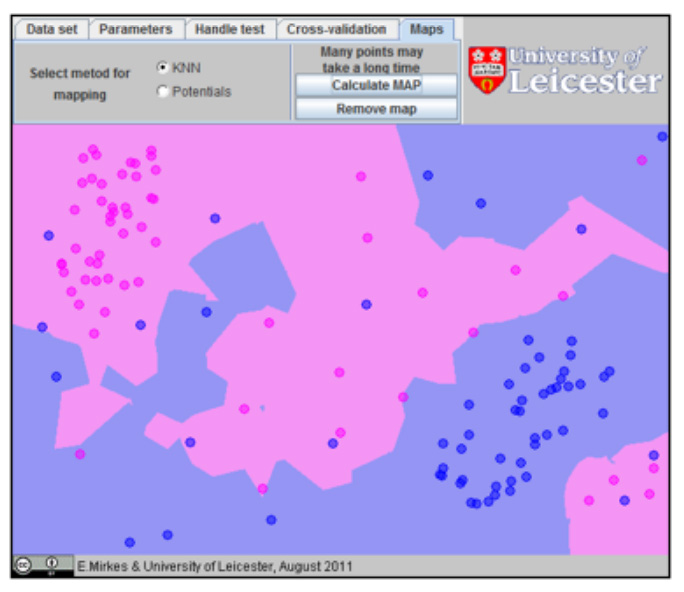
\includegraphics[scale = 0.5]{fig/KNNfig.jpg}
		\caption{KNN field here one can see how the knn will divide the space up with to different classes \citep{introKNN}}
		\label{KNN fig}
	\end{center}
\end{figure}

\colorbox{red}{OUR IMPLEMENTATION WILL BE DESCRIBED HERE (STILL NEEDED!!)}
\section{MATLAB Application}
With all the mathematics behind the whole segmentation, feature extraction and classification parts, we realized that instead of having to manually manage each and every function, a more intuitive way of utilizing the whole setup was needed. This led to the production of a graphical user interface (GUI) consisting of different elements the user can interact with, in order to take a piece of sound, segment it, and then get an automatic classification.

\subsection{Graphical User Interface}
Figure \ref{app-gui} shows the GUI of the active application, in which a waveform has been loaded, segmented, and annotated using the implemented kNN classifier. Starting from the top left corner (rectangle 1), we have a plot of the loaded signal. When this signal has been segmented, either automatically or manually, a set of vertical lines will be plotted to show the segmentation of the waveform. Along with the segmentation, the below plot (rectangle 3) will contain the change in the log-energy ($log(RMS)$), which should show a peak for each segment above. When the segments have been classified, the results will be presented in the table (rectangle 6) with one cell for each segment. To load the unclassified signal into the application the user must choose one of two options: load a sound file or make a new recording. This is done in the top right of the GUI (rectangle 2). Pressing the "Load wave" button will present the user with a file dialog, so a sound file can be located in a directory. The "Start recording" and "Stop recording" buttons will turn on and off the microphone to receive some input. When the sound is loaded a playback button will play the sound for the user. Before the classification, the user must choose the features used in the process. On the middle right side of the GUI (rectangle 4) is where features can be checked and their analysis window size and skip can be adjusted. Finally, below the features (rectangle 5) the user can load a manually segmented (and annotated) dataset for the classifier. Pressing "Load train data" will prompt the user to choose a sound file first, and then a text file containing the segmentation info (such as a segments start-point, duration and annotation). When the features above are chosen and adjusted the classifier can be trained using the "Train" button and finally the signal can be classified from the "Classify" button.

\begin{sidewaysfigure}
\begin{center}
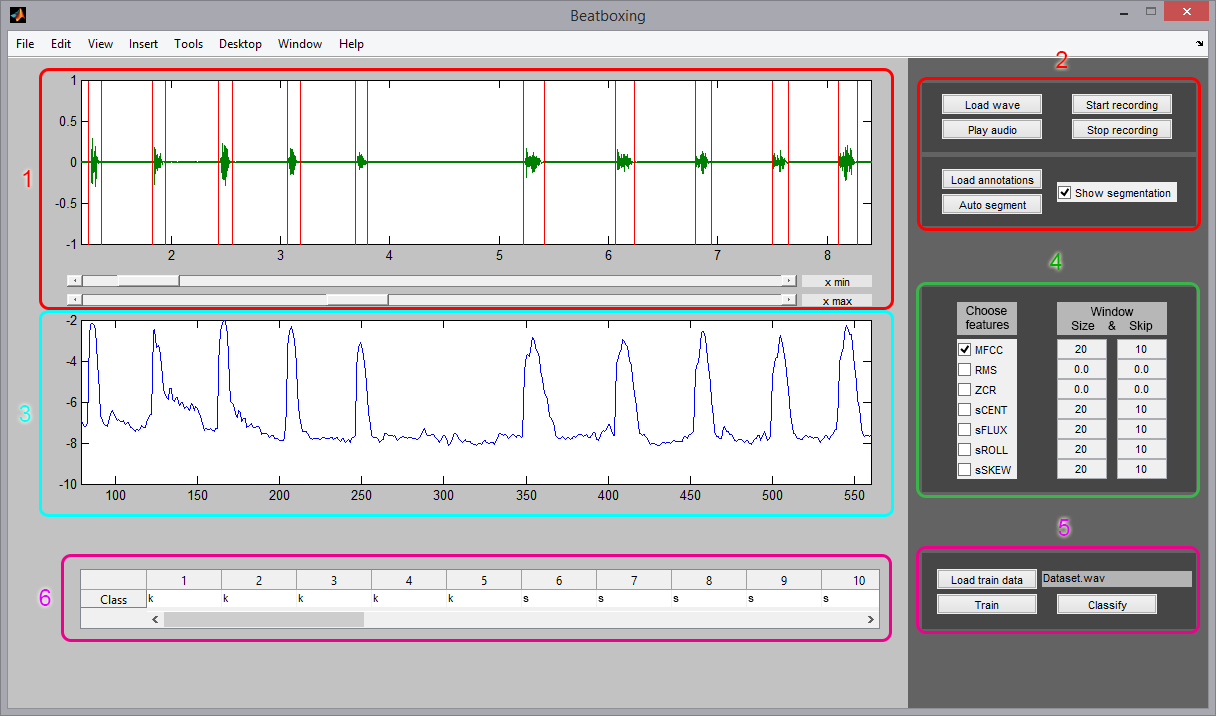
\includegraphics[width=\textwidth]{fig/Application.png}
\caption{Screenshot of the application GUI.}
\label{app-gui}
\end{center}
\end{sidewaysfigure}

\subsection{Application Workflow}
When the user starts the application the flow has to follow a specific path from taking an unclassified signal, segment it, and then automatically classify each sound included. The flow of the application is presented in figure \ref{app-flowchart}. To use the application one has to load a waveform of some recording of a person beatboxing, be it the user or someone else. This waveform then has to be segmented to identify the points at which each beatboxing sound (e.g. a kick drum or hi-hat) starts and ends. This process can either be done manually by the user or it automatically with the built-in segmentation algorithm. The manual process of segmenting the waveform has been explained in section \ref{sec:data-collecting} about data collection using Sonic Visualiser. The automatic segmentation uses the implementation described above.

\begin{figure}
\begin{center}
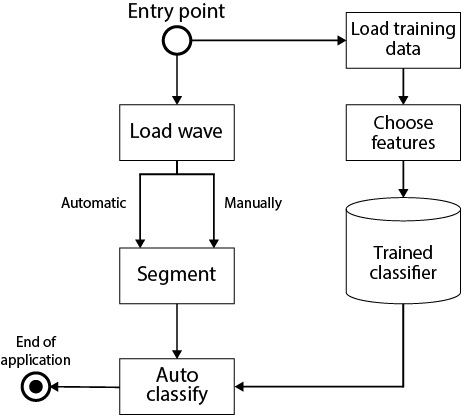
\includegraphics[scale=0.6]{fig/Application_flowchart.png}
\caption{Flowchart of the application.}
\label{app-flowchart}
\end{center}
\end{figure}

Before classifying these segments, the classifier has to be trained. To do this we start by loading a dataset that has been manually segmented. This dataset is a recording of multiple instances of the different beatboxing sounds used for the classification. When this dataset is loaded and segmented, the user must choose which features to use during the classification process. As an example we could choose MFCC using an analysis window size of 16 ms and a window skip of 8 ms. The classifier will then analyse all segments in the training dataset based on their MFCC and then store these analysis results to be used when classifying the unknown waveform.

When the user query a classification of the input waveform the classifier will take each segment from the input and compare it to the stored training data. Each segment will through this process get an annotation, i.e. a classification id, telling the user what kind of sound that segment has been interpreted as. A sequence of these annotation could be: \textit{k k k hh k s}, where the three first segments are classified as kicks followed by a hi-hat and then a snare.

Hereafter the user can adjust chosen features or choose new features to train the classifier again, and/or a new waveform can be loaded into the application and segmented to be classified as well.